\chapter{Rýchly úvod}
Aby sme mohli rýchlo začať programovať,
spravíme si základnú kostru programu. Čo v nej je si vysvetlíme neskôr, zatiaľ
ju budeme používať bez vysvetlenia:

\begin{lstlisting}
#include <iostream>
using namespace std;
int main() {
  // aj riadok začínajúci sa // je komentár
  // tu bude náš program
}
\end{lstlisting}


Na spustenie sa dá použiť nejaké prostredie (napr.
\link{https://www.codeblocks.org/}{Code::Blocks}, \link{https://visualstudio.microsoft.com}{MS Visual Studio}, ...), alebo linuxový terminál.  V
hocijakom editore (napr. %\link{https://atom.io/}{Atom}
\link{https://bluefish.openoffice.nl/index.html}{Bluefish},
\link{https://kate-editor.org/}{Kate},...) napíš súbor s
programom, ktorý nazvi napr. \vb{program.cc} a skompiluj ho napr. tak, že
v termináli napíšeš \vb{g++ program.cc -o program}. Týmto hovoríš
kompilátoru\footnote{% 
  Kompilátor je program, ktorý z textu programu vyrobí
  spustiteľný kód. V linuxe sú najrozšírenejšie kompilátory \vb{g++} a
  \vb{clang++}. Samozrejme, kompilátor je program, ako každý iný a treba ho mať
  nainštalovaný, aby fungoval.  } 
\vb{g++}, aby zobral program \vb{program.cc}
a vyrobil spustiteľný súbor (binárku) \vb{program}. Potom môžeš spustiť
\vb{./program} Keby program mal chybu, kompilátor vypíše chybovú hlášku a
binárku nevyrobí.  Keby si napríklad namiesto \prg!using! napísal
\prg!fusakla!, chybová hláška by mohla vyzerať nejak takto:

\begin{outputBox}
program.cc:2:1: \textcolor{red}{error:} ‘fusakla’ does not name a type
    2 | \textcolor{red}{fusakla} namespace std;
      | \textcolor{red}{^~~~~~}
\end{outputBox}

Vidíme, že chyba je v súbore \vb{program.cc} na riadku 2 a nasleduje aj opis chyby.
Prostredia ako Code::Blocks chybu zvyčajne vypíšu v samostatnom okne a zvýraznia v texte
programu. Ak je v riadku \vb{//}, zvyšok riadku kompilátor nečíta, môžeš si tam písať poznámky. Ak chceš mať komentár na viac riadkov, dá sa dať medzi 
oddeľovače \vb{/* komentár */}.
Keď už vieš, ako program skompilovať a spustiť, môžeme začať programovať.

\indexItem{Prg}{výraz a príkaz}
Základný stavebný prvok programu je {\em výraz}. Výraz je príklad, ktorý
sa počas behu programu vyráta a zistí sa jeho výsledok ({\em hodnota výrazu}). 
Napr. \prg~3*(2+5)~ je
výraz, ktorého hodnota (výsledok) je \prg~21~.  Druhý stavebný prvok je {\em príkaz}.
Príkaz hovorí, čo sa má s hodnotou výrazu urobiť. 
Príkaz je vždy ukončený bodkočiarkou.  Najjednoduchší
príkaz nerobí nič: \prg~3*(2+5);~ hovorí \cmd{Vypočítaj príklad $3\cdot(2+5)$ a
výsledok zahoď.} \indexItem{Prg}{výpis na \vb{cout} }Príkaz na vypísanie hodnoty na konzolu je \prg~cout<<~ takže
\prg~cout << 3*(2+5);~ znamená \cmd{Vypočítaj príklad $3\cdot(2 + 5)$ a výsledok
vypíš.} Špeciálny výraz je \prg ~endl~, ktorého hodnota je 'koniec riadku'.

Náš prvý program vyzerá takto:

\begin{lstlisting}
#include <iostream>
using namespace std;
int main() {
  cout << 3 * (2 + 5);
  cout << endl;
}
\end{lstlisting}

Keď ho spustíš, vypíše sa \vb{21}.

\indexItem{Prg}{premenná}
\indexItem{Prg}{typ \vb{int}}
Samozrejme nechceme, aby sme pre každý príklad písali samostatný program, ale chceme,
aby jeden program rátal veľa rôznych príkladov. Na to slúžia {\em premenné}. Premenná
je krabička, ktorá má meno a môže v nej byť uložená nejaká hodnota. Každú premennú treba
najprv vyrobiť a pritom treba povedať, aké hodnoty v nej môžu byť uložené (tomu sa hovorí
{\em typ} premennej). Základný typ je \prg~int~. Premenné typu \prg~int~ vedia ukladať celé 
čísla ({\em integer}). Meno typu je zároveň aj príkaz na vyrobenie premennej.
Takže \prg~int x;~ je príkaz, ktorý hovorí \cmd{Vyrob premennú, ktorá sa bude volať 
\prg~x~ a budú sa v nej dať ukladať celé čísla.} Premennú si môžeš nazvať hocijako, ale
meno sa musí skladať z veľkých a malých písmen (bez diakritiky) a podčiarkovníkov (\vb{\_}).
Môžu v ňom byť aj čísla, ale nesmie sa číslom začínať. Napr. \vb{u3\_prachDoma} je
dobré meno premennej. \indexItem{Prg}{priradenie}Príkaz \prg~=~ slúži na uloženie
výsledku do premennej. Takže \prg~x = 3 * (2 + 5);~ hovorí \cmd{Vypočítaj príklad $3\cdot(2+5)$
a výsledok ulož do premennej, ktorá sa volá \prg~x~}. Po vykonaní tohto príkazu
teda v premennej \prg~x~ bude uložená hodnota \prg~21~. Samotné meno premennej
je výraz (t.j. príklad), ktorého hodnota (t.j. výsledok) je číslo, 
ktoré je v nej práve uložené. Čo urobí nasledovný program?

\begin{lstlisting}[label=uvod.1]
#include <iostream>
using namespace std;
int main() {
  int x;
  x = 2 + 5;
  cout << 3 * x; @\ll1@
  cout << endl;
  x = 9 - 5; @\ll2@
  cout << 3 * x; @\ll3@
  cout << endl;
}
\end{lstlisting}

Prvý príkaz na riadku~4 vyrobí premennú \prg~x~, príkaz na riadku~5
vyráta príklad $2+5$ a výsledok (teda $7$)
uloží do premennej \prg~x~. Príkaz na riadku~\ref{uvod.1-1} ráta príklad 
\cmd{Vynásob číslo $3$ a obsah premennej
\prg~x~}. V premennej \prg~x~ je práve uložená sedmička, takže výsledok príkladu je 
$3\cdot7=21$ a to je číslo, ktoré sa vypíše a vzápätí sa vypíše koniec riadku.
Nasledujúci príkaz na riadku~\ref{uvod.1-2} do premennej \prg!x! uloží výsledok príkladu $9-5$, teda $4$. 
Príkaz na riadku~\ref{uvod.1-3} ráta to isté, čo príkaz na riadku~\ref{uvod.1-1}, t.j.
\cmd{Vynásob číslo $3$ a obsah premennej \prg!x!}. Teraz je ale v premennej \prg!x! uložené
číslo $4$, takže výsledok príkladu je $12$.


Posledný príkaz z tejto časti je \indexItem{Prg}{vstup z \vb{cin}}
\prg~cin>>~, ktorý čaká, kým na klávesnici napíšeš číslo (a stlačíš \vb{Enter})
a toto číslo uloží do premennej. Koľko vypíše nasledovný program,
ak mu napíšeš číslo 4? Skús si to najprv vyrátať sám a potom vyskúšať, či si mal pravdu. 

\begin{lstlisting}
#include <iostream>
using namespace std;
int main() {
  int x;
  cin >> x;
  x = x + 5;
  cout << 3 * x;
  cout << endl;
}
\end{lstlisting}

Zopakujme si to. Výraz je príklad, ktorý má výsledok (hodnotu). Videli sme
v ňom vystupovať sčítanie, odčítanie, násobenie, čísla a mená premenných. 
Keď sa počíta výsledok a vo výraze je meno premennej, zoberie sa hodnota, ktorá je v nej 
práve uložená. Toto je dôležité: musíme rozlišovať, medzi tým, čo vieme v čase, keď píšeme 
\indexItem{Alg}{compile-time vs runtime}
program ({\em compile-time}) a tým, čo vie program, keď už pracuje ({\em runtime}).
Napr. ak v predchádzajúcom programe  zadáme číslo 4, vypíše sa $3\cdot(4+5)$, teda $27$.
Ak zadáme číslo $1$, vypíše sa $3\cdot(1+5)$, teda $18$. Pri písaní programu vieme,
že ak napíšeme na vstupe hocijaké číslo $a$, pred výpisom bude v premennej \prg!x! uložená
hodnota $a+5$, a preto sa vypíše  výsledok príkladu $3\cdot(a+5)$.
Nevieme ale dopredu povedať, aké číslo bude v premennej \prg!x! uložené, to bude známe až počas behu programu.

\begin{column}{0.8}
\begin{uloha}
  Máme obdĺžnik z kamienkov ako na obrázku vpravo.
  Napíš program, ktorý prečíta zo vstupu dve čísla: koľko kamienkov je v riadku
  a koľko v stĺpci obdĺžnika. Program má vypísať, koľko kamienkov je v celom obdĺžniku.
  Obrázok vyššie má 5 kamienkov v riadku a 3 riadky a je v ňom  15 kamienkov.
\end{uloha}
\end{column}
\begin{column}{0.2}
  \vspace*{2ex}
  \centerline{
    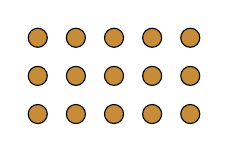
\begin{tikzpicture}[scale=0.8]
    \foreach \i in {0,...,4} \foreach \j in {0,...,2} {
     \filldraw[fill=brown!90!yellow] (\i*4ex,\j*4ex) circle (1ex);
    }
    \end{tikzpicture}}
\end{column}

